\section{Applying HDM on Testnet}
\nblink{brats/22a\_testnet\_hdm\_circles\_fixed.ipynb}

\begin{figure}[H]
    \centering
    \begin{subfigure}{.33\textwidth}
        \centering
        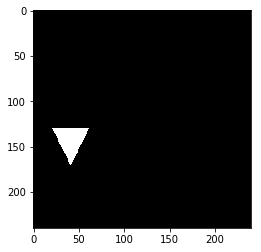
\includegraphics[width=\linewidth]{chapters/06_hdm/testnet/0.png}
        \caption{TODO}
    \end{subfigure}%
    \begin{subfigure}{.33\textwidth}
        \centering
        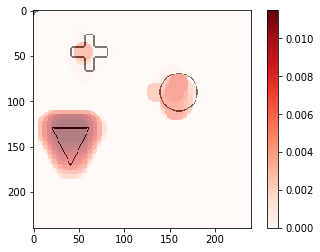
\includegraphics[width=\linewidth]{chapters/06_hdm/testnet/2.png}
        \caption{TODO}
    \end{subfigure}
        \begin{subfigure}{.33\textwidth}
        \centering
        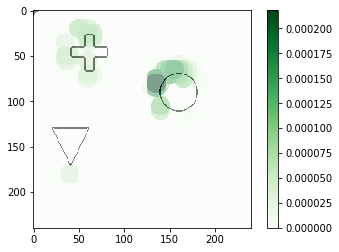
\includegraphics[width=\linewidth]{chapters/06_hdm/testnet/3.png}
        \caption{TODO}
    \end{subfigure}
    \caption{TODO}
\end{figure}

\begin{figure}[H]
    \centering
    \begin{subfigure}{.33\textwidth}
        \centering
        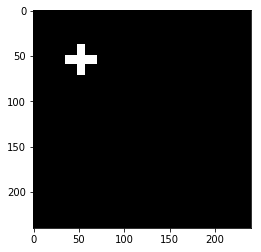
\includegraphics[width=\linewidth]{chapters/06_hdm/testnet/4.png}
        \caption{TODO}
    \end{subfigure}%
    \begin{subfigure}{.33\textwidth}
        \centering
        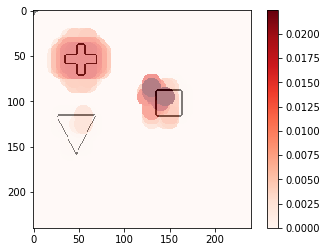
\includegraphics[width=\linewidth]{chapters/06_hdm/testnet/6.png}
        \caption{TODO}
    \end{subfigure}
        \begin{subfigure}{.33\textwidth}
        \centering
        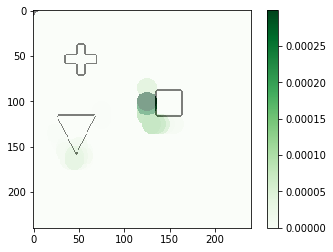
\includegraphics[width=\linewidth]{chapters/06_hdm/testnet/7.png}
        \caption{TODO}
    \end{subfigure}
    \caption{TODO}
\end{figure}

\begin{figure}[H]
    \centering
    \begin{subfigure}{.33\textwidth}
        \centering
        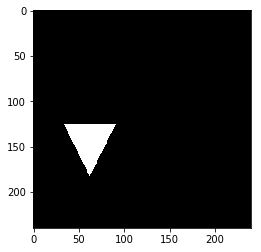
\includegraphics[width=\linewidth]{chapters/06_hdm/testnet/8.png}
        \caption{TODO}
    \end{subfigure}%
    \begin{subfigure}{.33\textwidth}
        \centering
        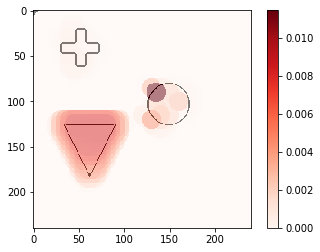
\includegraphics[width=\linewidth]{chapters/06_hdm/testnet/10.png}
        \caption{TODO}
    \end{subfigure}
        \begin{subfigure}{.33\textwidth}
        \centering
        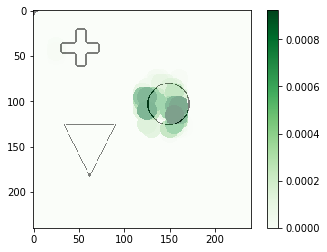
\includegraphics[width=\linewidth]{chapters/06_hdm/testnet/11.png}
        \caption{TODO}
    \end{subfigure}
    \caption{TODO}
\end{figure}
